%Erstemal, dass ich mit Latex arbeite, daher bitte nicht schlagen :D
\documentclass[a4paper, 11pt]{report}

\usepackage[ngerman]{babel}
\usepackage[latin1]{inputenc}
\usepackage{graphicx}
\usepackage{amsmath}
\usepackage{txfonts}
\usepackage{pstricks}
\usepackage{multirow}
\usepackage{stmaryrd}
\usepackage{wasysym}
\usepackage{enumerate}

\newcommand{\N}{\varmathbb{N}}
\newcommand{\Z}{\varmathbb{Z}}
\newcommand{\Q}{\varmathbb{Q}}
\newcommand{\R}{\varmathbb{R}}
\newcommand{\C}{\varmathbb{C}}
\newcommand{\F}{\varmathbb{F}}
\newcommand{\md}[1]{\text{mod }#1}		%sowie \mod{x} blo� ohne Leerzeichen vorne -> bei Klammern benutzen

\newcommand{\entspricht}{\stackrel{\scriptscriptstyle\wedge}{=}} %equivalent
\begin{document}

\tableofcontents

\newpage
\chapter{Einf�hrung}
\section{Inhalt}
�bertragung (Speicherung) von Daten:\\
Schutz vor:
\begin{itemize}
	\item[-] zuf�lligen oder systematischen (physikalischen bedingten) St�rungen
	\item[-] Abh�ren, absichtliche Ver�nderung von Dritten (Kryptologie / Verschl�sselung)
\end{itemize}
\underline{Kryptologie:}
\begin{itemize}
	\item[-] symmetrische Verfahren
	\item[-] asymmetrische Verfahren (Public-Key Verfahren)
	\item[-] Authentifizierung
	\item[-] Signaturen
\end{itemize}
\underline{Codierungstheorie}
\begin{itemize}
	\item[-] Fehlererkennung und Fehlerkorrektur
	\item[-] lineare Blockcodes
	\item[-] Decodierverfahren
\end{itemize} %Einführung
\chapter{Kryptologie}

\section{Grundbegriffe und einfache Verfahren}
\begin{figure}[h]
	\centering
	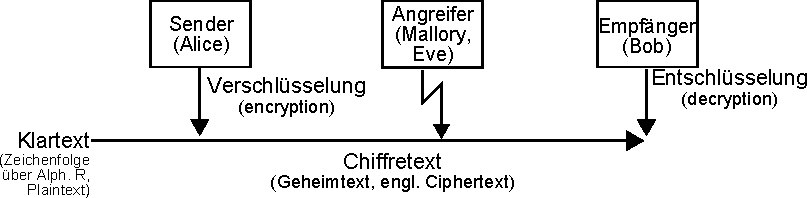
\includegraphics{./img/krypto_schaubild.pdf}
	\caption{Schaubild der Kryptologie}
	\label{img:Schaubild}
\end{figure}

\subsection{Verschl�sselung erfordert}

\begin{itemize}
	\item[-] Verschl�sselungsverfahren, Algorithmus (Funktion)
	\item[-] Schl�ssel $k_{e}$ (encryption key)
\end{itemize}

\[
	E(m,k_e)=c
\]	
$E$=Verschl�sselungs Funktion, $m$=Klartext, $c$=Chiffretext
\[
	E(m_1,k_e) \neq E(m,k_e)\ fuer \ m_1 \neq m_2
\]
\[
	D(c,k_d)=m
\]	
($k_d$ zu $k_e$ geh�riger Dechiffrierschl�ssel!)\\
$k_d=k_e$ (oder $k_d$ leicht aus $k_e$ zu berechnen):\\
\textbf{symmetrisches Verschl.verf.}, ansonsten \textbf{asymm. Verschl.verf.}. Ist $k_d$ nur sehr schwer (oder garnicht) zu $k_e$ berechenbar, so kann $k_e$ ver�ffentl. werden:\\
\textbf{Public-Key-Verfahren}.

\subsection{Beispiel f�r (nicht sicheres) symm. Verfahren}

\begin{itemize}
	\item[a)] $R=S=\left\{0,1,\ldots,25\right\}$\\
	Verfahren: Verschiebechiffre\\
	Schl�ssel: $i \in \left\{0,1,\ldots,25\right\}$\\
	Verfahren $ x \in \R \longrightarrow x+i\, mod\, 26=y$\\
	$y\longmapsto y-i\, mod\, 26 = y$\\
	$m=x_1 ... x_2 \longrightarrow  c = (x_1 + i\, mod\, 26) \textbf{}\ldots (x_n +i\, mod\, 26)$, $E(m,i)$\\
	Unsicher, weil Schl�sselmenge klein ist (Brute Force Angriff).
	\item[b)] R,S, Schl�sselmenge=Menge aller Permutationen von $\left\{1,\ldots,25\right\}=S_{26}$\\
	Verschl.: W�hle Permuation $\pi$\\
	$x \in \R \longrightarrow \pi (x)=y$\\
	Entschl.: $y \longrightarrow \pi^{-1}(y)=x$\\
	$m=x_1 \ldots x_r \rightarrow c=\pi(x_1)\ldots\pi(x_r)$\\
	$\begin{pmatrix}
  0 & 1 & 2 & \ldots & 25 \\
  3 & 17 & 4 & \ldots & 13
	\end{pmatrix}
	\longrightarrow \pi(0)=3$, u.s.w.\\
	Anzahl der Permutationen: $\left|{S_{26}}\right|=26!\approx4\cdot10^{26} \longrightarrow$ Brute-Force Angriff nicht mehr m�glich! \\
	Warum? Man muss im Schnitt 50\% der Permutationen testen. Angenommen man k�nnte $10^12$ Perm. pro Sekunde testen.\\
	Aufwand: $2\cdot10^{14}$ Sekunden $\approx 6.000.000$ Jahre\\
	Trotzdem unsicher!\\
	Grund: Charakteristiches H�ufigkeitsverteilung von Buchstaben in nat�rlichspr. Texten.
\end{itemize}
Verfahren beinhalten viele Verschl�sselungsm�glichkeiten, abh�ngig von der Auswahl des Schl�ssels.\\
Verfahren bekannt, aber Schl�ssel $k_d$ geheim!\\
\subsection{Prinzip von Kerkhoffs (1835-1903)}
Sicherheit eines Verschl�sselungsverfahren darf nicht von der Geheimhaltung des Verfahrens, sondern nur von der Geheimhaltung des verwendeten Schl�ssels abh�ngen!
%
%	Ende Stunde vom 29.10.2009
%
\\\\
Kryptologie besteht aus Kryptographie (Entwurf) und der Kryptoanalyse (Angriff).
Angriffserfolge:
\begin{itemize}
	\item[-] Schl�ssel $k_d$ wird gefunden
	\item[-] Eine zu der Dechiffrierfunktion $D(\cdot,k_d)$ �quivalente Funktion finden ohne Kenntnis von $k_d$
	\item[-] gewisste Chiffretexte werden entschl�sselt
\end{itemize}
\subsection{Arten von Angriffen}
\begin{itemize}
	\item[-] Ciphertext-Only Angriff
	\item[-] Known-Plaintext Angriff
	\item[-] Chosen-Plaintext Angriff
	\item[-] Chosen-Ciphertext Angriff
\end{itemize} %Kryptologie
\chapter{One-Time-Pad und perfekte Sicherheit}

Lauftextverschl�sselung
\\
Alphabet $\Z_k=\{0,1,\ldots,k-1\}$\\
In $\Z_k$ kann man addieren und multiplizieren mit $mod\,k$.\\
Klartext $x_1,x_2,\ldots,x_n$\\
Schl�sselwort $k_1,k_2,\ldots,k_n$\\
$x_1 + k_1\, mod\, k$, $x_n + k_n\, mod\, k \leftarrow$ Chiffretext\\
Mit nat�rlichsprachlichen Texten ist das Verfahren unsicher.\\
$\Z_2=\{0,1\}$, $1 \oplus 1 = 0 = 0 \oplus 0$, $0 \oplus 1 = 1 = 1 \oplus 0 \Rightarrow XOR$\\
Klartext in $\Z_2^n=\{(x_1,\ldots,x_n):x_i \in \Z_2\}$
Schl�ssel: Zufallsfolge �ber $\Z_2$ der L�nge $n$. $m$ Klartext, $k$ Zufallsfolge (beide L�nge $n$)\\
$c=m\oplus k$, $(x_1,\ldots,x_n)\oplus(k_1,\ldots,k_n):=(x_1\oplus k_1,\ldots,x_n\oplus k_n)$\\
\section{One-Time-Pad}
Schl�ssel $k$ darf nur einmal verwendet werden!\\
\[
	m_1\oplus k=c_1, m_2 \oplus k=c_2,c_1\oplus c_2=m_1\oplus k \oplus m_2\oplus k=m_1\oplus m_2
\]
Wieder nur Lauftext $\rightarrow$ unsicher!\\
$m_1$ und $m_2$ l�sst sich ermitteln.\\
Zufallsfolge der L�nge $n$: eigentlich unsinniger Begriff. Da jedes Bit unabh�ngig von anderen mit Wahrscheinlichkeit $\frac{1}{2}$ erzeugt wird (Output einer bin�r symmetrischen Quelle)\\
Jede Folge der L�nge $n$ ist gleich wahrscheinlich (Wahrscheinlichkeit $\frac{1}{2} n$\\
One-Time-Pad ist perfekt sicher.
\section{Perfekte Sicherheit}
Ein Verschl�sselungsverfahren ist perfekt sicher, falls gilt: F�r jeden Klartext $m$ und jedem Chiffretext $c$ (der festen L�nge $n$)\\
$pr(m|c)=pr(m)$\\
$pr(m|c)\rightarrow$ A-posteriori-Wahrscheinlichkeit (Wahrscheinlichkeit, dass $m$ Klartext, wenn $c$ empfangen wurde)\\
$pr(m)\rightarrow$ A-priori-Wahrscheinlichkeit\\
\textbf{Beispiel:} Substitutionschiffre aus Kapitel 2.\\
$n=5, m=HALLO, pr(m)>0$\\
Ang:$c=QITUA$ wird empfangen, $LL\neq TU \rightarrow pr(m|c)=0$\\
nicht perfekt sicher.\\
One-Time-Pad ist perfekt sicher. \\
(Bayes'sche Formel) $m\oplus k$\\
Jede Folge $c$ l�sst sich mit geeignetem $k$ in der Form $c=m\oplus k$ erhalten.\\
W�hle $k=m\oplus c$, $m\oplus k=m\oplus m \oplus c=c$\\
Bei gegebenem $m$ und zuf�llige gew�hlten Schl�ssel $k$ ist jeder Chiffretext gleichwertig. %One-TimePad und perfekte Sicherheit
\chapter{Symmetrische Blockchiffre}
\section{Blockchiffre}
Zerlege Klartext in Bl�cke (Strings) der L�nge $n$.  Jeder Block wird einzeln verschl�sselt (in der Regel wieder in einem Block der L�nge $n$). Gleiche Bl�cke werden gleich verschl�sselt.\\
Wieviele Blockchiffren der L�nge $n$ gibt es?\\
Alphabet $\Z_2=\{0,1\}$\\
$|\{\underbrace{(0,\ldots,0)}_{Block},(0,\ldots,1),\ldots,(1,\ldots,1)\}| = 2^n$\\
Blockchiffre = Permuation der $2^n$ Bl�cke.\\
$(2^n)!$ Blockchiffre\\
Wenn alle verwendet werden:\\
Schl�ssel = Permuation der $2^n$ Bl�cke\\
$(x_{1,1},\ldots,x_{1,n},x_{2,1},\ldots,x_{2,n},\ldots)$ \ \ \fbox{$n\cdot 2^n$ Bit}\\
Zur Speicherung eines Schl�ssels werden $n \cdot 2^n$ Bit ben�tigt.\\
Zum Beispiel:\\
$n=64, \ 64 \cdot 2^{64}=2^{70}\approx$ 1 ZetaByte $\approx$ 1 Milliarde Festplatten � 1 TB\\
\textbf{Illusional!}\\
Konsequenz:\ Verwende Verfahren, wo nur ein kleiner Teil der Permutation als Schl�ssel verwendet wird und so sich die Schl�ssel dann in k�rzerer Fom darstellt.
%
% Ende zweiter Vorlesung
% %Symmetrische Blockchiffre
\chapter{Affin-lineare Chiffre}

\section{Vorbemerkung}

\subsection{$n\times m$-Matrix}

\[
\begin{pmatrix}
	a_{11} & \ldots & a_{1m} \\
	\vdots &  & \vdots \\
	a_{n1} & \ldots & a_{nm}
\end{pmatrix}
\]

$1 \times n$ = Zeilenvektor = $(a_1,\ldots,a_m)$

$n \times 1$ = Spaltenvektor = $\begin{pmatrix} b_1 \\ \vdots \\ b_n \end{pmatrix}$

z.B. $a_{ij} \in \R,\ a_{ij} \in \Z$ oder $a_{ij} \in R,\ R$ Ring

$n \times m$-Matrix A,B
\[
\begin{pmatrix}
	a_{11} & \ldots & a_{1m} \\
	\vdots &  & \vdots \\
	a_{n1} & \ldots & a_{nm}
\end{pmatrix}
+
\begin{pmatrix}
	b_{11} & \ldots & b_{1m} \\
	\vdots &  & \vdots \\
	b_{n1} & \ldots & b_{nm}
\end{pmatrix}
:=
\begin{pmatrix}
	a_{11}+b_{11} & \ldots & a_{1m}+b_{1m} \\
	\vdots &  & \vdots \\
	a_{n1}+b_{n1} & \ldots & a_{nm}+b_{nm}
\end{pmatrix}
\]
\[
A=n\times m,\ B = m \times k,
\]
\[
A \cdot B
\begin{pmatrix}
	c_{1l} & \ldots & c_{1k} \\
	\vdots &  & \vdots \\
	c_{m1} & \ldots & c_{mk}
\end{pmatrix}
=
n\times k
\]
\[
c_{1l}=(a_{i1} \cdot b_{ij})+(a_{i2} \cdot b_{2j}) + \ldots + (a_{im} \cdot b_{mj})
\]
\[
(A+B)\cdot C = A\cdot B + B\cot C
\]

Im Allgemeinem: $A\cdot B \neq B\cdot A$\\

\subsection{Quadritsche Matrix ($n\times n$)}

\[
E_n=\begin{pmatrix}
	1 & \ldots & 0 \\
	\vdots & \ddots & \vdots \\
	0 & \ldots & 1
\end{pmatrix}
\]
\[
A=n\times n,\ A \cdot E_n=E_n \cdot A = A
\]
$A\ n\times n$-Matrix �ber kommutativen Ring R mit Eins.\\
Wann existiert Matrix $A^{-1}$(Inverse Matrix) mit $A^{-1} \cdot A = A \cdot A^{-1} = E_n$?\\
$det(A) \in R$\ Determinante von A\\
\\
$2\times 2$-Matrix: $det\begin{pmatrix}
	a_{11} & a_{12} \\ a_{21} & a_{21}
\end{pmatrix}
= a_{11} \cdot a_{22} - a_{12} \cdot a_{21}$\\
\\
\\
A besitzt inverse Matrix $\Leftrightarrow det(A)$ in R ein inverses besitzt\\
(z.B. R K�rper, $\Z ,\Q ,\Z_p,\ det(A)\neq 0$\\
\[
A^{-1}=
\begin{pmatrix}
	\frac{1}{det(A)}\cdot b_{11} & \ldots & \frac{1}{det(A)}\cdot b_{1m} \\
	\vdots & & \vdots \\
	\frac{1}{det(A)}\cdot b_{n1} & \ldots & \frac{1}{det(A)}\cdot b_{nm}
\end{pmatrix}
\]
$b_{ij}=(-1)^{i+j}$\ $det(A_{ji})$\\
\\
$A_{ji}=(n-1)\times (n-1)$-Matrix, die aus $A$ durchstreichen der $j$-ten Zeile und $i$-ten Spalte entsteht.
\[
A=
\begin{pmatrix}
	a_{11} & a_{12} \\ a_{21} & a_{22}
\end{pmatrix}\ \
A^{-1}=
\begin{pmatrix}
	a_{22} & -a_{12} \\ -a_{21} & a_{11}
\end{pmatrix}
\]
$R=\Z_k \ \{0,1,\ldots,k\}$\\
Addition und Multiplikation in $\Z_k (\oplus,\odot)$\\
normale Add. und Mult. mit $mod\, k$\\

\section{Affin-lineare Chiffren}
Klartextalphabet = Chiffretextalphabet = $\Z_k$ ($k=2,\ k=26$)\\
W�hle $n \times n$-Matrix $A$ �ber $\Z_k$ und Zeilenvektor $b$ der L�nge $n$ �ber $\Z_k$. Dies wird der Schl�ssel sein f�r die Chiffrierung.\\
Blockchiffre der L�nge $n$. Block = Zeilenvektor der L�nge $n$ �ber $\Z_k$.
Klartextblock $v$\\
Chiffretextblock $v \cdot A + b =: w$\\
$v \rightarrow v \cdot A +b =:w$
$w-b=v \cdot A$
ben�tigen: $A^{-1}$ existiert (d.h. $ggT(det(A),k)=1$)\\
Dechiffrierung: $(w-b)\cdot A^{-1} = v \cdot A \cdot A^{-1} = v \cdot E_n = v$\\
(wenn immer b=0 gew�hlt wird, dann lineare Chiffren, Hill-Chiffren)\\
Beispiel:\\
\[
A=
\begin{pmatrix}
	1 & 3 \\ 3 & 2
\end{pmatrix}
\ \Z_6
\]
Blockchiffre der L�nge $n$
$det(A)=1 \cdot 2 - 3 \cdot 3 = -7 = 5$ inverse in $\Z_6$
\[
\frac{1}{det(A)}=det(A)^{-1}=5
\]
\[
A^{-1}=5\cdot
\begin{pmatrix}
	2&-3\\-3&1
\end{pmatrix}
=
\begin{pmatrix}
	10&-15\\-15&5
\end{pmatrix}
=
\begin{pmatrix}
	4&3\\3&5
\end{pmatrix}
\]
Test: 
\[
A \cdot A^{-1} = 
\begin{pmatrix}
	1 & 3 \\ 3 & 2
\end{pmatrix}
\cdot
\begin{pmatrix}
	4&3\\3&5
\end{pmatrix}
=
\begin{pmatrix}
	4+9&3+15\\12+6&9+10
\end{pmatrix}
=
\begin{pmatrix}
	1&0\\0&1
\end{pmatrix}
\]
Verschl�sselung:

Schl�ssel:
$A = 
\begin{pmatrix}
	1 & 3 \\ 3 & 2
\end{pmatrix}
$ $b=(3,5)$

Klartextblock: $(1,2)$

Chiffretextblock: 
\[w=(1,2) \cdot 
\begin{pmatrix}
	1 & 3 \\ 3 & 2
\end{pmatrix}
+
(3,5)= (1,1)+(3,5) = (4,0)\]

Entschl�sselung:
\[ (w-b) \cdot A^{-1} = (1,1) \cdot 
\begin{pmatrix}
	4 & 3 \\ 3 & 5
\end{pmatrix}
=(1,2)
\]

$\Z_2 : n^2 + n$ Bit zur Speicherung eines Schl�ssels.

Wieviele inverse Matrizen �ber $\Z_2$ mit $n=64$?

$(2^{64}-1) \cdot (2^{64}-2) \cdot \ldots \cdot (2^{64}-2^{63}) \approx 0.29 \cdot 2^{4096}$

Verfahren ist unsicher gegen�ber Known-Plaintext-Angriffe.

$(A,b)$ Schl�ssel, A inverse $n \times n$-Matrix �ber $\Z_k ,b \ \in \Z_k^n$

Angenommen Angreifer kennt $n+1$ Klartext/Chiffretextpaare verschl�sselt mit $(A,b),\ v_0, v_1,\ldots,v_n \ w_0,\ldots,w_n$

Dann kann er haufig $(A,b)$ bestimmen.

$V=
\begin{pmatrix}
	v_1-v_0\\v_2-v_0\\\vdots\\v_n-v_0
\end{pmatrix}
\ n \times n$-Matrix

Angenommen: V ist invertierbar. Setze $W=
\begin{pmatrix}
	w_1-w_0\\\vdots\\w_n-w_0
\end{pmatrix}$
\[
V \cdot A =
\begin{pmatrix}
	(v_1-v_0) \cdot A \\ \vdots \\(v_n-v_0) \cdot A
\end{pmatrix}
=
\begin{pmatrix}
	v_1 \cdot A + b - v_0 \cdot A +b \\ \vdots \\
	v_n \cdot A + b - v_0 \cdot A + b
\end{pmatrix}
=
\begin{pmatrix}
	w_1-w_0\\ \vdots\\w_n-w_0
\end{pmatrix}
=W
\]

$V \cdot A$ bekannt, also auch $V^{-1}$:

$A=V^{-1} \cdot w$

$b=w_0 - v_0 \cdot A$

Beispiel: $n=2,\ k=25 \ \ \{A,\ldots, Z\}=\{0,\ldots,25\}$

\begin{center}
\texttt{HERBST} $\longrightarrow$ \texttt{NEBLIG}

\begin{tabular}{l|l|l}
H & 7 & \multirow{2}{*}{$v_0$} \\
E & 4 & \\
\hline
R & 17 & \multirow{2}{*}{$v_1$} \\
B & 1 & \\
\hline
S & 18 & \multirow{2}{*}{$v_2$} \\
T & 19 &
\end{tabular}
$\longrightarrow$
\begin{tabular}{l|l|l}
N & 13 & \multirow{2}{*}{$w_0$} \\
E & 4 & \\
\hline
B & 1 & \multirow{2}{*}{$w_1$} \\
L & 11 & \\
\hline
I & 8 & \multirow{2}{*}{$w_2$} \\
G & 6 &
\end{tabular}
\end{center}
\[
V=
\begin{pmatrix}
	10 & -3 \\
	11 & 15
\end{pmatrix}
=
\begin{pmatrix}
	10 & 23\\
	11 & 15
\end{pmatrix}, \
W=
\begin{pmatrix}
	14 & 7 \\
	21 & 2
\end{pmatrix}
\]
\[
det(V) = 10 \cdot 15  + 33 = 183 \equiv 1 (mod\ 26)
\]
\[
V^{-1}=
\begin{pmatrix}
	15 & 3 \\
	-11 & 10 	
\end{pmatrix}
=
\begin{pmatrix}
	15 & 3 \\
	15 & 10 	
\end{pmatrix}
\]
\[
A=V^{-1} \cdot W =
\begin{pmatrix}
	15 & 3 \\
	15 & 10 	
\end{pmatrix}
\cdot
\begin{pmatrix}
	14 & 7 \\
	21 & 2
\end{pmatrix}
=
\begin{pmatrix}
	210+63 & 105+6 \\
	210+210 & 105+20
\end{pmatrix}
=
\begin{pmatrix}
	13 & 7\\
	4 & 21
\end{pmatrix}
\]
\[
b=w_0-v_0 \cdot A = (13,4) - (7,4) \cdot 
\begin{pmatrix}
	13 & 7\\
	4 & 21
\end{pmatrix}
=
(10,1)
\]

Test:
\[
v_1 \cdot A + b= w_1, v_2 \cdot A + b= w_2
\]
 %Affin-Lineare Chiffre
\chapter{Der Advanced Encryption Standard (AES)}
\section{Mathematische Methoden gebraucht fuer AES} % NEED BETTER TITLE HERE
Seit 70er Jahren gab es DES (Blockl\"ange 64 Bit, Schl\"ussell\"ange 56 Bit) \\
\\
Nachfolger des DES: Daemen, Rijmen (Belgier)\\
Rijndael-Verfahren $\rightarrow$ AES (2002 FIPS 197)\\
\\
Iterierte Blockchiffre\\
Version mit 128 Bit Block und Schl\"ussel\"ange. \\
\\
$<$BILD VON EINER RUNDE VON AES KOMMT HIER HIN$>$\\
\\
Vorbemerkung: 128-Bit Bl\"ocke werden dargestellt als:\\
$\begin{pmatrix}
	a_{01} & a_{02} & \ldots & a_{03} \\
	a_{10} & a_{11} & \ldots & a_{13}\\
	\vdots & \vdots  & \vdots & \vdots \\
	a_{30} & \ldots  & \ldots & a_{33}
\end{pmatrix}$\\
\\
Jedes $a_{ij}$ = Byte\\
128er Block $\entspricht a_{00}a_{10}a_{20}\ldots a_{01}a_{11}\ldots a_{33}$ (spaltenweise gelesen)\\
\\
endlicher K\"orper: einfachste M\"oglichkeit $\Z_p$ ($p$ Primzahl)\\
$\F_{2^8}$ K\"orper mit $2^8 = 256$ Elementen\\
\\
Menge: Polynome vom Grad $< 8$ \"uber $\Z_2$\\
$b_7x^7 + \ldots + b_1x + b_0, b_i \in \Z_2 \\
(b_7, b_6, \ldots, b_0)$ Byte\\
\\
Addition = normale Addition von Polynomen\\
Multiplikation = normale Multiplikation von Polynomen + Reduktion modulo \\
irreduzibler Polynom vom Grad 8. ($x^8 + x^4 + x^3 + x + 1$)\\
\\
Bsp.\\
$(x^7 + x + 1) \odot (x^3 + x) = x^{10} + x^8 + x^4 + x^3 + x^2 + x\\
\\x^{10} + x^8 + x^4 + x^3 + x^2 + x$ mod $x^8 + x^4 + x^3 + x + 1\\
\\
x^{10} + x^8 + x^4 + x^3 + x^2 + x \div x^8 + x^4 + x^3 + x + 1 = x^2 + 1\\
\underline{x^{10} + x^6 + x^5 + x^3 + x^2}\\
\hspace*{8.85mm} x^8 + x^6 + x^5 + x^4 + x\\
\hspace*{8.85mm}\underline{ x^8 + x^4 + x^3 + x + 1} \\
\hspace*{16mm} x^6 + x^5 + x^3 + 1 \leftarrow \\
\\
(x^7 + x + 1) \odot (x^3 + x) = x^6 + x^5 + x^3 + 1$\\
\\
In $\F_{2^8}$ hat jedes Element $\neq$ 0 ein Inverses bzgl. $\odot$:\\
\indent $g \neq 0. Ex. g^{-1} \in \F_{2^8} : g \odot g^{-1} = 1$\\
\\
Erweiterte Euklid. Algo. f\"ur Polynome: \\
$g \neq 0$ (Grad $\leq 7$) \ \ $h = x^8 + x^4 + x^3 + x + 1$ irred. \ \ ggT($g, h$) = 1 \\
\\
EEA: $u,v \in \Z_2[x] : u \cdot g + v \cdot h = 1 \\
u$ mod $h =: g^{-1} \\
g^{-1} \odot g = ((u$ mod $h) \cdot g)$ mod $h = u \cdot g$ mod $h = (1 - vh)$ mod $h = 1$ mod $h = 1$\\
\section{SubBytes-Transfer}
$S_{i-1} =
\begin{pmatrix}
	a_{01} & a_{02} & \ldots & a_{03} \\
	a_{10} & a_{11} & \ldots & a_{13}\\
	\vdots & \vdots  & \vdots & \vdots \\
	a_{30} & \ldots  & \ldots & a_{33}
\end{pmatrix} , a_{ij}$ Bytes\\
Sei $g$ eines dieser Bytes, $g = (b_7b_6\ldots b_0), b_i \in \Z_2$\\
\\
1. Schritt: \ \
Fasse $g$ als Element in $\F_{2^8}$ auf.\\
\indent Ist $g = (0, \ldots, 0)$, so lasse g unver\"andert.\\
\indent Ist $g \neq (0, \ldots, 0)$, so ersetzte $g$ durch $g^{-1}$.\\
\\
2. Schritt: \ \ Ergebnis nach Schritt 1: $\tilde{g}$ wird folgenderm. Transformiert\\
\indent $\tilde{g} \cdot A + b = \tilde{\tilde{g}}$ \ \ (affin-lin. Transformation)
($\tilde{g}$: g-schlange, $\tilde{\tilde{g}}$:g-doppel-schlange)\\
\\
$A = 
\begin{pmatrix}
	1 & 1 & 1 & 1 & 1& 0 & 0 & 0\\
	0 & 1 & 1 & 1 & 1& 1 & 0 & 0\\
	\\
	\\
\end{pmatrix} \rightarrow$ zykl. Shift der vorherigen Zeile um 1 Stelle nach rechts.\\
\\
$b = \begin{pmatrix}
	1 & 1 & 0 & 0 & 0 & 1 & 1 & 0
\end{pmatrix}$\\
\\
Shritt 1 und 2 werden kombiniert, nicht jedes mal berechnet. Alle m\"oglichen Shifts ($2^8$ viele) sind in einer 16x16 Matrix und wird per Table-Lookup nachgeschlagen.\\
$g = (b_7b_6b_5b_4b_3b_2b_1b_0) \ \  b_7b_6b_5b_4$ = 0 bis 15 (Zeile) \ $b_3b_2b_1b_0$ (Spalte)

\section{Shift Rows Transformation}
4x4-Matrix von Bytes: 
$\begin{pmatrix}
	Erste\ Zeile\ unveraendert\\
	1\ stelle\ nach\ links\ zykl.\\
	2\ stellen\ nach\ links\ zykl.\\
	3\ stellen\ nach\ links\ zykl.\\
\end{pmatrix}$

\section{Mix Columns Transformation}
4x4-Matrix, Eintr\"age als Elemente in $\F_{2^8}$ auffassen.\\
Multiplikation von links mit Matrix
(Mult. der Eintr. in $\F_{2^8}):
\begin{pmatrix}
	x & x+1 & 1 & 1\\
	1 & x & x+1 & 1\\
	1 & 1 & x & x+1\\
	x+1 & 1 & 1 & x\\
\end{pmatrix}\\
x \entspricht
\begin{pmatrix}
	0 & 0 & 0 & 0 & 0 & 0 & 1 & 0\\
\end{pmatrix}$

\section{Schl\"usselerzeugung}
Ausgangsschl\"ussel hat 128 Bit. (16er String in Hexcode)\\
\\
Schreibe als 4x4-Matrix von Bytes. 4 Spalten $w(0), w(1), w(2), w(4)$. Definiere weitere 40 Spalten \`a 4 Bytes.\\
\\
$w(i-1)$ sei schon definiert.

$ 4 \nmid i : w(i) := w(i-4) \oplus w(i-1)$ (byteweise XOR)\\
$ 4 \mid i : w(i) := w(i-4) \oplus T(w(i-1))$ (T Transformation)\\
T?\\ $w(i-1) =
\begin{pmatrix}
	a\\
	b\\
	c\\
	d\\
\end{pmatrix} , \ a,\ldots,d Bytes$\\
Wende auf $b, c, d, a$ SubBytes-Transformation an $\rightarrow e, f, g, h$ $(b \rightarrow e)$\\ 
$r(i) =
\begin{pmatrix}
	0 & 0 & 0 & 0 & 0 & 0 & 1 & 0\\
\end{pmatrix}^{\frac{(i-4)}{4}}$ Potenz. in $\F_{2^8}$\\
$T(w(i-1)) = 
\begin{pmatrix}
	e \oplus r(i)\\
	f\\
	g\\
	h\\
\end{pmatrix}$\\
Rundenschl\"ussel $K_i$: 4x4-Matrix mit Spalten $w(4i), w(4i+1), w(4i+2), w(4i+3)$\\
\\
(Nebenbemerkung: Linear heisst $f(x+y) = f(x) + f(y)$)
 %AES
\chapter{Public-Key-Systeme}
\section{Grundidee}
Diffie, Hellman, 1976
Jeder Teilenehmer hat ein Paar von Schl�sseln:
\begin{itemize}
	\item[-] �ffentlichen Schl�ssel $P_A$
	\item[-] geheimen Schl�ssel $G_A$
\end{itemize}
Zu $P_A$ geh�rt �ffentlich bekannte Verschl�sselungsfunktion $E_{P_A}$ (=$E(\cdot, P_A$)\\
$B\stackrel{m}{\rightarrow}A: E_{P_A}(m)=c$
\begin{enumerate}
	\item $m$ darf mit "realistischen Aufwand" nicht aus $E_{P_A}(m)$ berechenbar sein. $E_{P_A}$ ist \textbf{Einwegfunktion}\\
	($E_{P_A}$ muss effizient berechenbar sein, aber $E_{P_A}^{-1}$ nicht!)
	\item $A$ muss mit Hilfe einer Zusatzinformation (=$G_A$) in der Lage sein, $E_{P_A}^{-1}$ effizient zu berechnen.
	\[
	D_{G_A}(c)=m=E_{P_A}^{-1}(c)
	\]
	Injektive Einwegfunktionen, die mit Zusatzinformation effizient invertierbar sind: \textbf{Geheimt�rfunktion} (trapdoor function)
\end{enumerate}

Aus 1) und 2) folgt:
\begin{enumerate}
	\item[3] $G_A$  darf aus $P_A$ nicht schnell berechenbar sein!
\end{enumerate}
Es ist unbekannt ob Einwegfunktion existieren! Notwendig f�r die Existenz von Einwegfunktionen:
\[
P\neq NP
\]
Es gibt Kandidaten f�r Einwegfunktionen.
\section{RSA-Verfahren} (Rivest, Shamir, Adleman, 1977)
Beruht auf Schwierigkeit gro�e Zahlen zu  faktorisieren!
\subsection{Schl�sseslerzeugung}
W�hle zwei gro�e Primzahlen $p,q (p\neq q)$ (mindestens 500 Bit L�nge)\\
Bilde $n=p\cdot q$\\
\[ \varphi(n)=\| \{a \in \N : 1 \leq a < n, ggt(a,n)=1\}\| \]
\[ n=p\cdot q : \varphi(n)=(p-1)\cdot (q-1) \]
[nicht teilerfremd zu $n$:$1\cdot p, 2 \cdot p,\ldots,(q-1)\cdot p = n = 1\cdot q, 2\cdot q,\ldots,(p-1)\cdot q$\\
$(p-1)+(q-1)+1$\\
$\varphi(n)=n-(p-1)-(q-1)-1=n-p-q+1=p\cdot q - p-q + 1 = (p-1)\cdot (q-1)$]\\
W�hle $e$, $1 < e < \varphi(n)$ mit $ggT(e,\varphi(n))=1$\\
Zufallswahl, bestimme $ggT(e,\varphi(n))$ mit Euklidischer Algorithmus, so lange, bis $e$ mit $ggT(e,\varphi(n))=1$ gefunden ist.)
\subsubsection{�ffentlicher Schl�ssel}
$(n,e)=P_A$\\
W�hle $d < \varphi(n)$ mit $e\cdot d \equiv 1 (mod\ n)$ (d.h. $\varphi(n) \mid e \cdot d -1, e\cdot d=1+k\cdot \varphi(n)$ f�r $k \in \N$)\\
(Wende erweiterten Euklidischen Algorithmus auf $e,\ \varphi(n)$ an:\\
Liefert $u,v \in \Z$ mit $u\cdot e + v\cdot \varphi(n)=ggT(e,\varphi(n))=1$\\
$d=u\ mod\ \varphi(n)$\\
$u\cdot e + v \cdot \varphi(n)\ mod\ \varphi(n)=1$\\
$( \underbrace{u\ mod\ \varphi(n)}_{d} \cdot e)  mod\ \varphi(n)=1$)
\subsubsection{Geheimerschl�ssel}
$G_A=d$
\subsection{Verschl�sselung}
$B$ Nachrichtan $A$. Codiere Nachricht als Zahl. Zerlege in Bl�cke deren Zahlwert $< n$. Sei $m$ so ein Block. $(m<n)$\\
$m^e\ mod n = c$
\subsection{Entschl�sselung}
$c^d mod n = m$\\
G�ltigkeit basiert auf kleinem Satz von Fermat:\\
$r$ Primzahl, $ggT(a,r)=1$ (d.h. $r \nmid a$)\\
$a^{r-1} \equiv 1 (mod\ r)$\\
Sei $m<n=p\cdot q$
\[
c=m^e\ mod\ n, c^d\ mod\ n=m^{e\cdot d}\ mod\ n
\]
\[
e \cdot d = 1 + k \cdot \varphi (n) = 1 + k \cdot (p-1) \cdot (q-1)
\]
Ist $p \nmid m$, so 
\[
m^{e\cdot d}=m^{1+k\cdot (p-1)\cdot (q-1)}=m\cdot =(m^{p-1})^{k\cdot (q-1)}\stackrel{mod\ p}{\Rightarrow} m\cdot 1^{k\cdot (q-1)} (mod\ p) = m (mod\ p)
\]
Ist $p \mid m$:
\[
m \equiv 0 \equiv m^{e\cdot d} (mod\ p)
\]
In jedem Fall:
\[
m^{e\cdot d} \equiv m (mod\ p)
\]
Genauso:
\[
m^{e\cdot d} \equiv m (mod\ q)
\]
\[
p \mid m^{e\cdot d} - m,\ q  \mid m^{e\cdot d} -m , p\neq q \Rightarrow n=p\cdot q \mid m^{e\cdot d}-m
\]
\[
m^{e\cdot d} \equiv m (mod\ n),\ m^{e\cdot d} mod\ n = m
\]
\subsubsection{Schnelle Berechnung von modularen Produkten}
\[
m^e\ mod\ n
\]
\[
e=\sum^k_{i=0} e_i \cdot z^k,\ e_i \in \{0,1\},e_k=1
\]
\[
m^e=m^{2\cdot k + e_{k-1}\cdot 2^{k-1}+\ldots+e_1\cdot 2+e_0}
\]
\[
( ( \ldots ( (m^2 \cdot m^{e_{k-1}} )^2 \cdot m^{e_{k-2} } )^2 \ldots )^2 \cdot m^{e_1} )^2\cdot m^{e_0}
\]
gel�st im worst case mit $2\cdot k$ Multiplikationen
\[
k=\left\lfloor log_2(e)\right\rfloor
\]
\fbox{Nach jedem Rechenschritt $mod\ n$ reduzieren!}

\section{Sicherheit vom RSA-Verfahren}
Falls $p,\ q$ bekannt $\Rightarrow \varphi(n),\ d$ bekannt.\\
$\varphi(n)$ bekannt $\Rightarrow\ p,\ q$ bekannt.\\
$\varphi(n)=n-q-p+1$ bekannt $\Rightarrow\ p+q=s$ bekannt, $p\cdot q=n$ bekannt.\\
$p\cdot (s-p)=n$ $p^2-s\cdot p + n = 0$ quadratische Gleichung f�r $p$
\paragraph{Es gilt auch:} Bestimmung von $d$ ist "`genauso schwierig"' wie die Faktorisierung von $n$.\\
Komplexit�t der besten Faktorisierungsalgorithmen:
\[
	O(e^{c\cdot (\log n)^{\frac{1}{3}}
	\cdot ((\log \log n)^{\frac{2}{3}})})
\]
Um eine 640 Bit Zahl zu faktorisieren braucht man 30-CPU-Jahre auf einer 2.2 GHz CPU.\\ \\
H�ufig wird $e=3$ gew�hlt.\\
\fbox{HIER KOMMT NOCH EINE GRAFIK HIN} %img
\\
$ggT(n_i,n_j)=1$
\begin{eqnarray*}
	c_1=m^3\ mod\ n_1\\	
	c_2=m^3\ mod\ n_2\\	
	c_3=m^3\ mod\ n_3
\end{eqnarray*}
Eve f�ngt $c_1,\ c_2,\ c_3$ ab: Chinesisches Restsatz:

\begin{eqnarray*}
	&0 \leq x \leq n_1,\ n_2,\ n_3\ \ \mbox{mit}\ x=c_i\ mod\ n_i&\\
	&i=1,2,3&\\
	&x\ \mbox{ist eindeutig bestimmbar}&\\
	&m^3 \equiv c_i\ mod\ n_i,\ m^3 < n_1,n_2,n_3&\\
	&\Rightarrow x=m^3 \Rightarrow m=\sqrt[3]{x}&
\end{eqnarray*}
Wenn $e=5$, dann braucht man 5 Nachrichten.

\subsection{Wie bestimmt man gro�e Primzahlen?}
\begin{eqnarray*}
	&p	\mbox{Primzahl},\ a\in \Z,\ ggT(a,p)=1&\\
	&a^{p-1} \equiv 1 (mod\ p)\ \mbox{[kl. Satz von Fermat]}&
\end{eqnarray*}
\textbf{gegeben:} $n,\ ggT(a,n)=1$ $a^{n-1} \equiv 1\ (mod\ n)$?\\
\subsection{Fermat-Test} Wenn nicht, so ist $n$ keine Primzahl. Wenn ja, so keine Aussage m�glich. W�hle neues a!\\
Es gibt zusammengesetze Zahlen $n$ (Carmichael-Zahlen) mit:
\begin{eqnarray*}
	&a^{n-1} \equiv 1\ (mod\ n)\ \forall\ a\ \mbox{mit}\ ggT(a,n)=1&
\end{eqnarray*}

\subsection{Miller-Rabin-Test}
\begin{eqnarray*}
	&ggT(a,p)=1&\\
	&p\ \mbox{Primzahl}\	p-1=2^s \cdot t,\ 2 \nmid t&\\
	&a^{2^s\cdot t} \equiv 1\ (mod\ p)&\\
	&(a^{2^{s-1} \cdot t})^2=b&\\
	&a^{2^{s-1} \cdot t} =\left \{
		\begin{matrix}
			1\ mod\ p \\ -1\ mod\ p
			
		\end{matrix}
	\right.&\\
	&b^2\equiv 1\ (mod\ p)&\\
	&(b\ mod\ p)^2=1 \in \Z_p&\\
	&x^2-1 \in \Z_p [x]&
\end{eqnarray*}	
\fbox{Entweder $a^t\equiv1\ (mod\ p)$ oder $a^{s^i\cdot t}\equiv -1\ (mod\ p)$ f�r ein $0 \leq i \leq s$}
Teste dies mit $n$ statt $p$.\\
Wenn $n$ keine Primzahl ist, dann gibt es mindestens $\frac{3}{4} \varphi(n)$ viele $a$, so dass der Test fehlschl�gt.\\
$\rightarrow$ probabilistischer Primzahltest\\
$p$ Primzahl $\Z_p^{*}=\Z_p \setminus \{0\}$ Gruppe bez�glich Multiplikation (zyklisch)\\
\begin{eqnarray*}
	&\exists g \in \Z_p^{*} : \{g^0,g^1,g^2,\ldots,g^{p-2}\}=\Z_p&\\
	&g^{p-1}\equiv 1\ (mod\ p)&
\end{eqnarray*}	
Primitivwurzel $mod\ p$\\
$0 \leq a \leq p-2:a\mapsto g^a\ mod\ p$ Kandidat f�r Einwegfunktion.\\
$g^a\ mod\ p \rightarrow a$ (diskreter Logarithmus) ist nach heutigem Stand schwer!\\
\subsection{Diffie-Hellman-Verfahren zur Schl�sselvereinbarung}
$A,\ B$ wollen gemeinsamen Schl�ssel $K$ f�r ein symm. Verfahren vereinbaren; es steht nur unsichere Kommuniaktionskanal zur Verf�gung.
\paragraph{L�sung:} $p, g$ (Bitl�nge von $p>$ Bitl�nge von $K$) (k�nnen �ffentlich bekannt sein).\\
\begin{enumerate}
	\item $A$ w�hlt zuf�llig $a\in \{2,\ldots,p-2\}$\\
	$A$ berechnet $x=g^a\ mod\ p$\\
	($a$ geheim halten)
	\item $B$ w�hlt zuf�llig $b\in \{2,\ldots,p-2\}$\\
	$B$ berechnet $y=g^b\ mod\ p$\\
	($b$ geheim halten)
	\item $A \stackrel{x=g^a}{\rightarrow} B$\\
	$B \stackrel{y=g^b}{\rightarrow} A$\\
	$A: y^a\ mod\ p = g^{b\cdot a}\ mod\ p = K$\\
	$B: x^b\ mod\ p = g^{a\cdot b}\ mod\ p = K$
\end{enumerate}
\subsection{Sicherheit}
Angreifer: $p,g,\ g^a\ mod\ p,\ g^b\ mod\ p$\\
gesucht: $g^{a\cdot b}\ mod\ p$\\
Einzig bekannte M�glichkeit ist das Berechnen $a$ aus $g^a:(g^b)^a\ mod\ p=K$ m�sste diskretes Logarithmus-Problem l�sen.
\subsection{Man-in-the-Middle}
$M$ f�ngt $g^a$ und $g^b$ ab und w�hlt $c \in \{2,\ldots,p\}$ und schickt $g^c\ mod\ p$ an $A$ und $B$.\\
$A:\ g^{c\cdot a}\ mod\ p,\ B:\ g^{c\cdot b}\ mod\ p$. Beide Schl�ssel kennt auch $M$
\section{ElGamal-Public Key Verfahren (1984)}
\subsection{Schl�sselerzeugung}
$A$ w�hlt $p,g$ wie bei Diffie-Hellmann. W�hlt $a \in \{2,\ldots,p-2\},\ x=g^a\ mod\ p$.\\
�ffentlicher Schl�ssel: $(p,g,x)$\\
Geheimer Schl�ssel: $a$
\subsection{Verschl�sselung}
Klartext $m:\ 1 \leq m \leq p-1$\\
$B \stackrel{m}{\rightarrow} A$ \\
$B$ w�hlt zuf�llig $b \in \{2,\ldots,p-2\}$\\
$y=g^b\ mod\ p$\\
Er berechnet $x^b\ mod p$ und $f=m\cdot x^b\ mod\ p$, sendet $(y,f)$ an $A$,
\subsection{Entschl�sselung}
$y^a\ mod\ p\ (= x^b\ mod\ p)$\\
Berechnet $(y^a)^{-1}\ mod\ p$ $[(y^a)^{-1}=(y^{\overbrace{p-1-a}^{\geq 0}})]$\\
$f\cdot (y^a)^{-1}\ mod\ p=m$
\subsubsection{Nachteil zu RSA}
Doppelte L�nge wird gebraucht, da Nachricht (Chiffre) und Teilschl�ssel versendet werden. %Public Key Systeme
\chapter{Signaturen, Hashfunktionen, Authentifizierung}
\section{Anforderung an digitale Signaturen}
\paragraph{Identit�tseigenschaft:}

ID des Unterzeichners des Dokuments wird sichergestellt
\paragraph{Echtheitseigenschaft:}

des signiertem Dokument

\paragraph{Verifikationseigenschaft:}

Jeder Empf�nger muss digitale Signatur verifizieren k�nnen.

\section{RSA-Signatur (vereinfachte Version)}

$A$ will Dokument $m$ signieren. \\
$A$ bestitzt �ffentlichen RSA-Schl�ssel $(n,e)$, geheimen Schl�ssel $d$.

Signatur: $m^d\ mod\ n$ sendet $(m,\ m^d\ mod\ n)$ an $B$.\\
$(m^d\ mod\ n)^e = m^{e \cdot d}\ mod\ n = m\ (mod\ n)$\\
$m < n$\\
Wenn $m^{e \cdot d}\ mod\ n = m$, dann akzeptiert $B$ die Signatur.\\
$m > n\ \ m^d\ mod\ n$ $B\ mod\ n$. Ist $m^{'}\ mod\ n = m\ mod\ n$, dann $(m^{'},m^d\ mod\ n)$ g�ltige Signatur.

\subsection{Wie lassen sich lange RSA-Signaturen vermeiden?}
\paragraph{Def:}

Sei $R$ ein endliches Alphabet.\\
\textbf{Hashfunktion} $H: \R^{*} \rightarrow R^k (k \in \N$ fest $)$ soll effizient berechenbar sein.

\section{RSA-Signatur mit HASH-Funktion}

$H$ �ffentlich bekannte Hashfunktion.\\
$A$ will Nachricht $m$ signieren.\\
Bildet $H(m)$ und signiert $H(m) : H(m)^d\ mod\ n$ sendet $(m, H(m)^d\ mod\ n)$\\
Verifikation durch $B$: $m \rightarrow H(m)$\\
$(H(m)^d\ mod\ n)^e\ mod\ n = H(m)$

\subsection{Angriffsm�glichkeiten}
\begin{description}
	\item[-] Angreifer kann $H(m)$ bestimmen wenn es ihm gelingt, $m' \neq m$ zu finden, so $(m', H(m)^d\ mod\ n)$ g�ltige Signatur von $m$ durch $A$.
	\item[-] Angreife w�hlt zuf�llig $y$ und berechnet $y^e\mod\ n = z$\\
	Gelingt es ihm, $m$ zu finden mit $H(m)=z$, dann ist $(m,y)$ g�tlige Signatur von $m$ durch $A$\\
	$H(m)\ \  y^e=H(m)$ 
\end{description}

\paragraph{Def:}

Eine \textbf{kryptographische Hashfunktion} ist eine Hashfunktion, die folgende Bedinungen erf�llt.
\begin{enumerate}
	\item $H$ ist Einwegfunktion (um Angriffe des zweiten Typs zu vermeiden)
	\item $H$ ist \textbf{schwach kollisionsresistent}, d.h. zu gegebenem $m \in R^{*}$, soll es effizient nicht m�glich sein ein $m' \neq m$, mit $H(m)=H(m')$, zu finden. (um Angriffe des ersten Typs zu vermeiden)
\end{enumerate}
Versch�rfung von 2.
\begin{enumerate}
	\item[$2'$] $H$ ist \textbf{stark kollisions resistent}, wenn es effizient nicht m�glich ist $m \neq m'$ zu finden, mit  $H(m) = H (m')$.
\end{enumerate}

Da $R^{*}$ unendlich und $\left| R^k \right|=\left|R\right|^k$ endlisch ist, existiert unendlich viele Paare $(m,m'),\ m\neq m'$ mit $H(m)=H(m')$.\\
(Bilde $\left|R\right|^k+1$ viele Hashwerte: Kollision)\\
Kollisionen lassen sich nicht vermeiden, sie sollten aber nicht schnell herstellbar sein.

\subsection{Satz: Geburtstagsparadoxon}

Ein Merkmal komme in $m$ verschiedenen Auspr�gungen vor. Jede Person besitze genau eine dieser Merkmalsauspr�gungen. Ist $c \geq \frac{1+\sqrt{1+8\cdot m \cdot \ln{2}}}{2} \approx 1.18 \sqrt{m}$, so ist die Wahrscheinlichkeit, dass unter $l$ Personen zwei die gleiche Merkmalsauspr�gung haben, mindestens $\frac{1}{2}$ (Geburtstage: $m=366, l=23$).

\paragraph{Beweis}

$l$ Personen\\
Alle M�glichkeiten $(g_1,g_2,\ldots,g_l), g_i \in \{1,\ldots,m\}$ $m^l$ M�glichkeiten.\\
Alle Merkmalauspr�gungen verschieden: $m \cdot (m-1) \cdot (m-2) \cdot \ldots \cdot (m-(l-1))$\\
Wahrscheinlichkeit, dass $l$ Personen lauter verschiedene Geburtstage haben.\\
\[
q = \frac{m \cdot (m-1) \cdot (m-2) \cdot \ldots \cdot (m-(l-1)}{m^l}=\prod^{l-1}_0{1 - \frac{i}{m}}
\]
Wann ist $q \leq \frac{1}{2}$?\\
$e^x \geq 1+x$\\
\[
\prod^{l-1}_0{1 - \frac{i}{m}}
\leq \prod^{l-1}_0{e^{-\frac{i}{m}}}
=e^{\prod^{l-1}_0{-\frac{i}{m}}}
=e^{- \frac{1}{m}\sum^{l-1}_0{i}}
=e^{- \frac{1}{m} \cdot \frac{l \cdot (l-1)}{2}}
\]
\[
\ln{a}\leq - \frac{1}{m} \cdot \frac{l \cdot (l-1)}{2} = - \frac{l^2-l}{2 \cdot m}
\]

\subsection{Hashfunktion}

$H(m) = H(m'), m \neq m'$\\
$H: \Z_2^* \rightarrow \Z_2^n$ ($2^n$ Hashwerte)\\
Bei Erzeugung von circa $2^\frac{n}{2}$ Hashwerten ist die Wahrscheinlichkeit,
dass zwei gleich sind ungef�hr $\frac{1}{2}$.\\ 
$n=64 : 2^{32}$ Hashwerte $(~4 \cdot 10^9)$ unsicher.\\
Weit verbreitet waren und sind:
\begin{itemize}
	\item[] MD5 (message digerst / Ron Rivest, 1991, 128 Bit)
	\item[] SHA-1 (Secure Hash Algorithm, NSA, 1992/1993, 160 Bit)
\end{itemize}

\section{Authentifizierung}

Nachweise bzw. �berpr�fung, dass jemand derjenige ist f�r den er sich ausgbit.\\
M�glichkeiten der Authentifizierung durch:
\begin{itemize}
	\item[] \textbf{Wissen}
	\item[] Besitz
	\item[] biometische Merkmale
\end{itemize}
g�ngiste Methode: Passwort \\
Im Allgemeinem: Passwort $w$ abgespeichert als $f(w)$ $f$ Einwegfunktion.\\
$w$ $f^n(w)=w_0 \stackrel{sicher}{\rightarrow}$ Id. �berpr�fer $f$ Einweg.
\begin{enumerate}
	\item Auth. $w_1=f^{n-1}(w) \rightarrow f(f^{n-1}(w))=w_0$ ersetzt $w_0$ durch $w_1$
	\item Auth. $w_2=f^{n-2}(w) \rightarrow \ldots$
\end{enumerate}

\fbox{Passwortsicherheit: http://www.schneier.com/crypto-gram-0701.html}

\section{Challenge-Response-Authentifizierung}
RSA-Verfahren
$A \stackrel{auth.}{\longrightarrow} B$\\
�ffentlicher Schl�ssel: $(n,e)$\\
geheimer Schl�ssel: $d$\\
$A \stackrel{Zufallszahl\ r}{\longleftarrow} B,\ r<n\ \leftarrow$ \textbf{Challenge}\\
$A \stackrel{r^d\ mod\ n}{\longrightarrow} B$ �berpr�ft, ob $r^{d^e}\ mod\ n = r\ \leftarrow$ \textbf{Response}\\
Damit $B$ sich sicher seien kann, dass es wirklich $A$ ist, kann $B$ so oft wie es f�r n�tig h�lt neue $r$ schicken und dadurch die Chance verringern, dass $A$ nicht $A$ ist. %Signaturen, Hashfunktionen, Authentifizierung
\chapter{Secret Sharing}
Geheimnis wird auf mehrere Teilnehmer verteilt (Teilgeheimnisse), so dass gewisse Teilmengen der Teilnehmer das Geheimnis mit ihren Teilgeheimnissen rekonstruieren k�nnen, die anderen nicht. \\ \\
$T$ = \{ $t_1, \ldots , t_n$\}, $k < n$ \ \ (T Menge der Teilnehmer) \\ \\
Jede Teilmenge von $T$ mit mindestens $k$ Teilnehmer sollen Geheimnis rekonstruieren k�nnen, Teilmengen von $T$ mit weniger als $k$ Teilnehmer nicht.\\
\section{($k, n$) - Schwellenwertsysteme}
1979 Shamir (How to share a secret)

\subsection{Konstruktion}
Vereinbarung von gro\ss er Primzahl $p$, mindestens $p >= n + 1$ %FORMATTING!!
\\
\\
$g \in \Z_p = \{0, \ldots , p-1\}$

\subsection{Verteilung der Teilgeheimnisse}
Dealer w\"ahlt zuf\"allig $a_1, \ldots, a_{k-1} \in \Z_p, a_{k-1} \neq 0, k =$ Schwelle \\
$f(x) = g + a_1x + \ldots + a_{k-1}x^{k-1} \in \Z_p[x] $ \\
$(a_1, \ldots , a_{k-1}$ h\"alt er geheim, nat\"urlich auch g)\\
\\
Dealer w\"ahlt zuf\"allig $x_1, \ldots, x_n \in \Z_p$ (paarweise verschieden). \\
Teilnehmer $t_i$ erh\"alt als Teilgeheimnis $(x_i, f(x_i))$ (Punkt auf Polynom)\\
Bei $x=0$ hast du $g$.

\subsection{Rekonstruktion(sversuch) des Geheimnisses}
$k$ Teilnehmer $(x_{i_1}, f(x_{i_1})), \ldots, (x_{i_k}, f(x_{i_k}))$ \\
Durch diese Punkte ist $f$ eindeutig bestimmt, z.B. durch Lagrange-Interpol.: \\
$f(x_{i_j}) = g_{i_j} \\
\\
f(x) = \sum_{j=1}^k g_{i_j} \cdot \frac{(x-x_{i_1}), \ldots, (x-x_{i_{j-1}})(x-x_{i_{j+1}}), \ldots, (x-x_{i_k})}
                      {(x_{i_j}-x_{i_1}), \ldots, (x_{i_j}-x_{i_{j-1}})(x_{i_j}-x_{i_{j+1}}), \ldots, ((x_{i_j}-x_{i_k})}\\
f(0) = g\\
g = \sum_{j=1}^k g_{i_j} \prod_{l=j} \frac{x_{i_l}}{(x_{i_l}-x_{i_j})}$ \\
Bei mehr als $k$ Teilnehmer selbe Ergebnis.\\
Weniger als $k$ Teilnehmer $(k')$: Anderes Polynom wegen weniger Punkte, also warscheinlich anderer $g$.\\
Erzeugen Polynom vom Grad $<= k' - 1$ \\ % FORMATTING
F\"ur alle $k \in \Z_p$ existiert gleich viele Polynome vom Grad $<= k'-1$ %FORMATTING
durch die vorgegebene $k'$ Punkte, die bei $h$ durch $y$-Achse gehen. %Secret Sharing Scheme
\chapter{Codierungstheorie}

\section{Grundbegriffe und einfache Beispiele}

\subsection{Codierung} (Kanalcodierung)\\
Sicherung von Daten/Nachrichten gegen zuf\"allig auftretenden Fehler bei Speicherung/\"Ubertragung.\\
\begin{figure}[h]
	\centering
	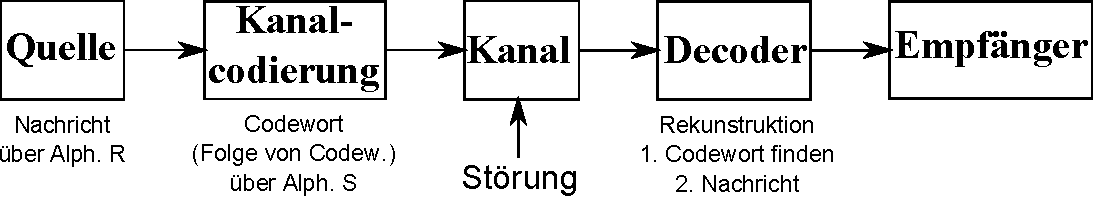
\includegraphics[totalheight=0.1\textheight]{./img/codierung_schaubild.pdf}
	\caption{Schaubild der Codierung}
	\label{img:Schaubild Codierung}
\end{figure}

\subsection{Ziele}
\begin{itemize}
	\item M\"oglichst viele Fehler erkennen und gegebenenfalls korrigieren. %ABKUERZUNG
	\item Aufwand f\"ur Codierung und Decodierung m\"oglichst gering.
\end{itemize}

\section{Grundprinzip} Hinzuf\"ugen von Redundanz\\
\\
Es gibt zwei Typen um Redundanz zu erzeugen.
\subsection{FEC-Verfahren (Forward Error Correction)}
Aufgetretene Fehler sollen erkannt \underline{und} korrigiert werden.\\
Vorteil: keine Verz\"ogerung der \"Ubertragung aber ggf. gro\ss e Redundanz notwendig.

\subsection{ARQ-Verfahren (Automatic Repeat Request)}
Aufgetretene Fehler sollen erkannt werden, werden nicht korrigiert. Stattdessen  wiederholt die \"Ubertragung beim Sender anfordern.\\
\\
Vorteil: geringe Redundanz, aber Verz\"ogerung.\\
\\
\subsubsection{Beispiele}
\begin{enumerate}
\item Parity-Check-Codes\\
z.B. Nachrichten: 00, 01, 10, 11\\
\\
Codierung: 00 $\rightarrow$ 000\\
01 $\rightarrow$ 011\\
10 $\rightarrow$ 101\\
11 $\rightarrow$ 110\\
(gerade Anzahl von Einsen in den Codew\"ortern)\\
\\
1 Fehler wird erkannt, nicht korrigiert.\\
2 Fehler werden nicht erkannt.

\item Wiederholungscode\\
Nachrichten wie in 1.\\
\\
Codierung: 00 $\rightarrow$ 000000
01 $\rightarrow$ 010101\\
10 $\rightarrow$ 101010\\
11 $\rightarrow$ 111111\\
(3-Fache Wiederholung)\\
\\
1 Fehler wird erkannt und korrigiert.\\
\underline{01}01\underline{01} $\rightarrow$ 010101 $\rightarrow$ 01
\item Nachrichten wie in 1.
Codierung: 00 $\rightarrow$ 00000\\
01 $\rightarrow$ 01101\\
10 $\rightarrow$ 10110\\
11 $\rightarrow$ 11011\\
\\
Je zwei Codew\"orter unterscheiden sich an mindestens 3 Positionen.\\
Angenommen 1 Fehler tritt bei \"Ubertragung auf. Dann gibt es genau ein Codewort, dass sich vom empfangenen Wort an genau einer Stelle unterscheidet; in das wird decodiert.\\
\\
Muss immer Ungerade unterschiede in Codew\"ortern sein. Bei 5 diffs sind 2 Fehler korrigierbar.
\item (ehmaliger) ISBN-Code
International Standard Book Number\\
\\
10-Stelliger Code\\
Erste 9 Ziffern haben inhaltliche Bedingung ($\entspricht$ Nachricht)\\
10. Ziffer: Pr\"ufziffer\\
\\
Beispiel: 3-540-26121-? (Land - Verlag - Buchnummer - Pr\"ufziffer)\\
\\
Uncodierte W\"orter sind gebildet \"uber $R=\{0, \ldots, 9\}$\\
Codierte W\"orter sind gebildet \"uber $S=\{0, \ldots, 9, X\}$\\
\\
ISBN-Wort $C_{10}C_9\ldots C_2C_1$\\
$C_{10}\ldots C_2$ inhaltliche Bedingung, $C_1$ wird so gew\"ahlt, dass
\[
	\sum^{10}_{k=1} k \cdot C_k \equiv 0 (\md 11)
\]

$10\cdot C_{10}+\ldots + 2\cdot C_2 + C_1 \equiv 0(\md 11)$ falls $C_1 = 10$ so setzte $C_1 = X$\\
$C_1$ vom Beispiel ausrechnen.\\
\\
$ 10\cdot 3+9\cdot 5+8\cdot 4+7\cdot 0+6\cdot 2+5\cdot 6+4\cdot 1+3\cdot 2+2\cdot 1+C_1 = 0 (\md 11)$\\
$ 161 + C_1 = 0 (\md 11) \Rightarrow C_1 = 4$\\
\\
\"Andern einer Ziffer wird erkannt:\\
$C_{10} C_9\ldots C_2 C_1 \rightarrow\ C_i$ wird $X_i \neq C_i$ ersetzt\\
$C_{10} \ldots C_{i+1} X_i C_{i-1} \ldots C_1$
\[
	\sum^{10}_{k=1, k \neq i} k \cdot C_k + i \cdot x_i = 
	\underbrace{\sum^{10}_{k=1, k \neq i} k \cdot C_k}_{\equiv 0 (\md 11)}
	\overbrace{
			\underset{\underset{\nequiv 0 (\md 11)}{\uparrow}}{i} 
			\cdot (\underbrace{x_i-c_i}_{\nequiv 0 (\md 11)}) 
	}^{\nequiv 0 (\md 11)}
	\nequiv 0(\md 11)	
\]
Fehler wird erkannt, Korrektur nicht m\"oglich.\\
\\
$3-540-26121-4 \equiv 0(\md 11)$\\ \\
$\left.
\begin{matrix}
	3-540-26121-\mathbf{6} \\
	3-540-2612\mathbf{2}-4
\end{matrix}
\right\} \text{Pr\"ufsumme 2.}
$\\

Vertauschung von Zwei Ziffern wird erkannt.\\
$C_i$ und $C_j$ vertauscht.\\
O.B.d.A $C_i \neq C_j$\\
$C_{10} \ldots \underset{\stackrel{\uparrow}{i}}{C_j} \ldots \underset{\stackrel{\uparrow}{j}}{C_i} \ldots C_1$\\
\[
	\sum^{10}_{k=1, k\neq i,j} k \cdot C_k + i \cdot 	C_j + j \cdot C_i
	= \sum^{10}_{k=1} k \cdot C_k + i(C_j-C_i)+j(C_i-C_j)
\]
\[
	= 
	\underbrace{\sum^{10}_{k=1} k \cdot C_k}_{\equiv 0 (\md 11)}
	 + 
	 \underbrace{(C_j-C_i)}_{\nequiv 0 (\md 11)}
	 \underbrace{(i-j)}_{\nequiv 0 (\md 11)}
	 \nequiv 0 (\md 11)
\]
Vertauschung wird durch gewichtete Quersummen erkannt.


\item EAN-13-Code\\
\\
European Article Number\\
13-Stelliger Code, erste 12 Ziffer sind inhaltlich festgelegt.\\
13. Ziffer ist Pr\"ufziffer.\\
$R=S=\{ 0, \ldots, 9\}$ \\
$C_1 \ldots C_{12}C_{13}$\\
\\
$C_1 \ldots C_{12}$ inhaltliche Angabe (in der Regel):\\
$C_1C_2$ Herstellerland (40-43 Deutschland)\\
$C_6 \ldots C_7$ Hersteller
$C_8 \ldots C_12$ interne Produktions Nummer\\
\\
$C_{13}$ so gew\"ahlt, dass\\
\[
	C_1 + 3\cdot C_2 + C_3 + 3\cdot C_4 + \ldots + 3\cdot C_{12} + C_{13} \equiv 0 (\md 10)
\]
$x \rightarrow 3x$ Permutation auf $\Z_{10} (\md 10)$, da ggT(3,10)=1\\ %FORMATTING vom ggT?
1 Fehler wird erkannt. Vertauschung in der Regel nicht erkannt. \\
\\
\"Ubersetzung in Barcode: \\
$C_1 C_2 \ldots C_7 C_8 \ldots C_{13}$\\
\\
Jede der Ziffern $C_2, \ldots, C_{13}$ wird durch einen 0-1-String der L\"ange 7 bin\"ar codiert. \\
$0 \entspricht$ wei�er Balken, $1 \entspricht$ schwarzer Balken. \\
Codierung sorgt daf\"ur, dass nie mehr als 4 wei�e oder schwarze Balken nebeneinander stehen. \\

\newpage

\begin{figure}[h]
	\centering
	
\includegraphics[totalheight=0.1\textheight]{./img/ean13.png}
	\caption{EAN-13 Barcode}
	\label{img:EAN-13 Barcode}
\end{figure}

Schmalen Balken in Mitte und am Rand, sind nur Abtrennzeichen, die nichts mit EAN zu tun haben und nur beim einscannen helfen.\\
5 zu $0110001_2$ \\
\\
$C_2,\ldots, C_7$ werden nach Code A oder Code B codiert. $C_1$ bestimmt welcher dieser beiden Codes verwendet wird. \\
$C_8,\ldots, C_{13}$ werden nach Code C codiert.\\
$C_1$ ergibt sich aus der Art der Codierung von $C_2,\ldots,C_7$

%Table shit here
\begin{center}
	\begin{tabular}{| c | c | c | c | p{2cm} |}
	\hline
	 &\multicolumn{2}{|c|}{\textbf{Ziffern $\mathbf{C_2 - C_7}$}} & \textbf{Ziffern $\mathbf{C_8 - C_{13}}$} & \textbf{bestimmt durch} $\mathbf{C_1}$ \\
	\hline
	\textbf{Zeichen} & \textbf{Code A} & \textbf{Code B} & \textbf{Code C} & \textbf{Code D}\\
	\hline
	\textbf{0} &	0001101 &	0100111 &	1110010 &	AAAAAA\\
	\textbf{1} &	0011001 &	0110011 &	1100110 &	AABABB\\
	\textbf{2} &	0010011 &	0011011 &	1101100 &	AABBAB\\
	\textbf{3} &	0111101 &	0100001 &	1000010 &	AABBBA\\
	\textbf{4} &	0100011 &	0011101 &	1011100 &	ABAABB\\
	\textbf{5} &	0110001 &	0111001 &	1001110 &	ABBAAB\\
	\textbf{6} &	0101111 &	0000101 &	1010000 &	ABBBAA\\
	\textbf{7} &	0111011 &	0010001 &	1000100 & 	ABABAB\\
	\textbf{8} &	0110111 &	0001001 &	1001000 &	ABABBA\\
	\textbf{9} &	0001011 &	0010111 &	1110100 &	ABBABA\\
	\hline
	\end{tabular}
\end{center}







Codew\"orter von Code A,B oder C kommen nur einmal vor. Daher treten nie mehr als 4 gleiche Balken nebeneinander auf. \\
\end{enumerate}




 %Codierung
\chapter{Blockcodes}
\[
\begin{matrix}
	00 & \rightarrow & 00000\\
	01 & \rightarrow & 01101\\
	10 & \rightarrow & 10110\\
	11 & \rightarrow & 11011
\end{matrix}
\]

\subsection{Definition}

$S$ endl. Menge (=Alphabet), $n \in \N$. \\
Ein Blockcode $\mathcal{C}$
der (Block-)L\"ange $n$ \"uber $S$ ist Teilmenge von $S^n=\underset{\longleftarrow \ \  n\ \  \longrightarrow}{S \times \ldots \times S}$ \\ % Pfeilspa� <- n -> \times
\\
Elemente von $\mathcal{C}$ hei�en \textbf{Codew\"orter}. \\
Ist $\left| S \right| = 2$ (i.d.R. $S=\lbrace 0,1 \rbrace$, so \textbf{bin\"ar} Code.\\
$\left| \mathcal{C} \right| = m$, so ist $m \leq \left| S \right| ^ n$. \\
\\
Dann lassen sich $n$ Informationssymbole (oder Strings von Informationssymbolen) codieren (Codierungsfunktion). Folge von Informationssymbolen (oder Strings) werden dann in Folge von Codew\"ortern codiert.

\subsection{Definition: Hamming-Abstand}
$S$ endl. Alphabet, $n \in \N$. \\
$a,b \in S^n$ $a=(a_1, \ldots, a_n)$, $b=(b_1, \ldots, b_n)$ \\
$d(a, b)= \sharp \lbrace i : a_i \neq b_i \rbrace$ \\
\textbf{Hamming-Abstand} von $a$ und $b$. \\
(Richard W. Hamming, 1915-1998, Begr\"under der Codierungstheorie)\\
\subsubsection{Eigenschaften}
\begin{description}
	\item[a)] $d(a,b)=0 \Leftrightarrow a=b$
	\item[b)] $d(a,b)=d(b,a)$
	\item[c)] $d(a,b) \leq d(a,c) + d(c,b)$ (Dreiecksungleichung) \\
					($a_i \neq b_i \Rightarrow a_i \neq c_i$ oder $b_i \neq c_i$) 
	\item[d)] Wenn $(S,+)$ komm. Gruppe, dann auch $S^n$\\
					$[ (a_1,\ldots a_n) + (b_1, \ldots b_n) = (a_1+b_1,\ldots, a_n+b_n)]$\\
					$d(a,b)=d(a+c,b+c)$ (Translationsinvarianz)				
\end{description}

Also: Wird $x \in \mathcal{C}$ gesendet und $y \in S^n$ wird empfangen und $d(x,y)=k$, so sind $k$ Fehler aufgetreten.
\subsection{Definition}
\subsubsection{a) Hamming-Decodierung}
f\"ur Blockcode $\mathcal{C} \subseteq$ $S^n$ \\
Wird $y \in S^n$ empfangen, so wird $y$ zu einem Codewort $x' \in \mathcal{C}$ decodiert, das unter allen Codew\"ortern minimalen Hamming-Abstand zu $y$ hat.\\
\[
	d(x',y)=min\  d(x,y), x \in \mathcal{C}
\]
($x'$ muss nicht eindeutig bestimmt sein)	\\
z.B. $\mathcal{C}$ $ = \{ (0000), (1111) \}$\\
Empfangen: $0011$ $x'$ nicht eindeutig in diesem Fall.\\
\\
($\left| S \right | = 2$: Hamming-Decodierung ist bestm\"oglich, falls jedes Symbol in einem Codewort mit der gleichen Wahrscheinlichkeit $p < \frac{1}{2}$ ver\"andert wird und wenn jedes Codewort gleich wahrscheinlich ist.)\\

\subsubsection{b) Minimalabstand}
$\mathcal{C}$ Blockcode in $S^n$, Minimalabstand von $\mathcal{C}$: \\
\[
	d(\mathcal{C}) = min \  d(x,x')\mathbf{,}\ \  x,x' \in \mathcal{C}, x \neq x'
\]

(Ist $\left| \mathcal{C} \right| = 1$, so $d(\mathcal{C})=n$)\\
$[Bsp: \mathcal{C} = \lbrace (00000),(01101),(10110),(11011) \rbrace , d(\mathcal{C})=3]$\\

\subsubsection{c)} 
Ein Blockcode $\mathcal{C}$ ist \textbf{t-Felder-korrigierend}, falls $d(\mathcal{C}) \geq 2t+1$, und er hei�t \textbf{t-Fehler-erkennend}, falls $d(\mathcal{C}) \geq t+1$. \\
\\
Begr\"undung f\"ur die Bezeichnung in c) \\
"`Kugel"' vom Radius $t$ um $x \in \mathcal{C}: K_t(x) = \{y \in S^n: d(x,y) \leq t\}$\\
\\
Ist $d(\mathcal{C}) \geq 2t+1$, so sind Kugelm vom Radius $t$ um Codew\"orter disjunkt. \\
\\
Angenommen es existiert $y \in S^n$ mit $y \in K_t(x)\cap K_t(x')$, $x,x' \in \mathcal{C}, x \neq x'$. Dann $d(x,x') \leq d(x,y)+d(y,x') \leq t+t = 2t$. Widerspruch\\ %LIGHTNING ARROW \lightning
$x \in \mathcal{C}$ gesendet, $y$ wird empfangen, und angenommen maximal $t$-Fehler sind aufgetreten, dann $y \in K_t(x)$ und Abstand zu jedem anderem Codewort ist $> t$\\
$\Rightarrow$ Hamming-Decodierung ist korrekt.\\
$d(\mathcal{C}) \geq t+1$ und es treten maximal $t$ minimal $1$ Fehler auf, so ist $y$ kein Codewort.\\
\\
\textbf{Bsp}: 
\begin{description}
	\item[a)] $n$-fach Wiederholungscode \\
	$
	\begin{matrix} 
		S_n & \rightarrow & \underset{\longleftarrow \ \ n \ \ \longrightarrow}{S_1 S_1 \ldots S_1} \\ 
		\vdots \\
		S_k & \rightarrow & \underset{\longleftarrow \ \ n \ \ \longrightarrow}{S_k S_k \ldots S_k}
	\end{matrix}$\\
	\\
	$\mathcal{C}=\lbrace (s,s,\ldots,s): s \in S \rbrace \subseteq S^n$ \\
	$d(\mathcal{C})=n$ \\
	\\
	$\left\lfloor \frac{n-1}{2} \right\rfloor$-Fehler-korr.
	\item[b)] ISBN, EAN-Codes, $d(\mathcal{C})=2$, 1-Fehler-erkennend.	
\end{description}
 %Blockcodes

\newpage
\end{document}
